\section{CMB Analyse}

% TODO Acronyms
Die Analyse des CMB Leistungsspektrums wird mit Hilfe der in einer 
Semesterarbeit entwickelte SHCL Library (zu finden auf Github unter 
\url{https://github.com/Darnor/SHCL}) durchgeführt.

\subsection{Was sind unsere Daten}
Als Datengrundlage wird erst das öffentlich verfügbare CMB Bild in 
Rektangularprojektion \ref{bib:cmb_public_equirectangular} verwendet.
% TODO: Image CMB (rectangular)
% TODO: Aufzeugung funktion der conversiation RBG -> "Kelvin"

\subsection{Das Leistungsspektrum}

% TODO: Erklärung C_l
% TODO: diff cosmic variance \Delta C_l und C_l

\subsection{Spärische harmonische Koeffizienten}
% TODO: c_l^m erklärung
% TODO: Problemstellung bei berechnung rauschen -> grosse zahl -> lösung

\subsection{Resultate}

Abbildung \ref{fig:cmb-power-spec-2500} zeigt, was wir mit unseren Berechnungen 
ein ähnliches Bild wie erwartet bekommen. Natürlich ist das ganze nicht 
perfekt, so stimmt die $l(l+1)C_l/2\pi$ Skala um rund einen Faktor 10 nicht mit 
dem erwarteten überein. Das alles macht deutlich, dass unsere Umwandlung der 
RGB Werte in Kelvin nicht ganz korrekt ist.

\begin{figure}
	\centering
	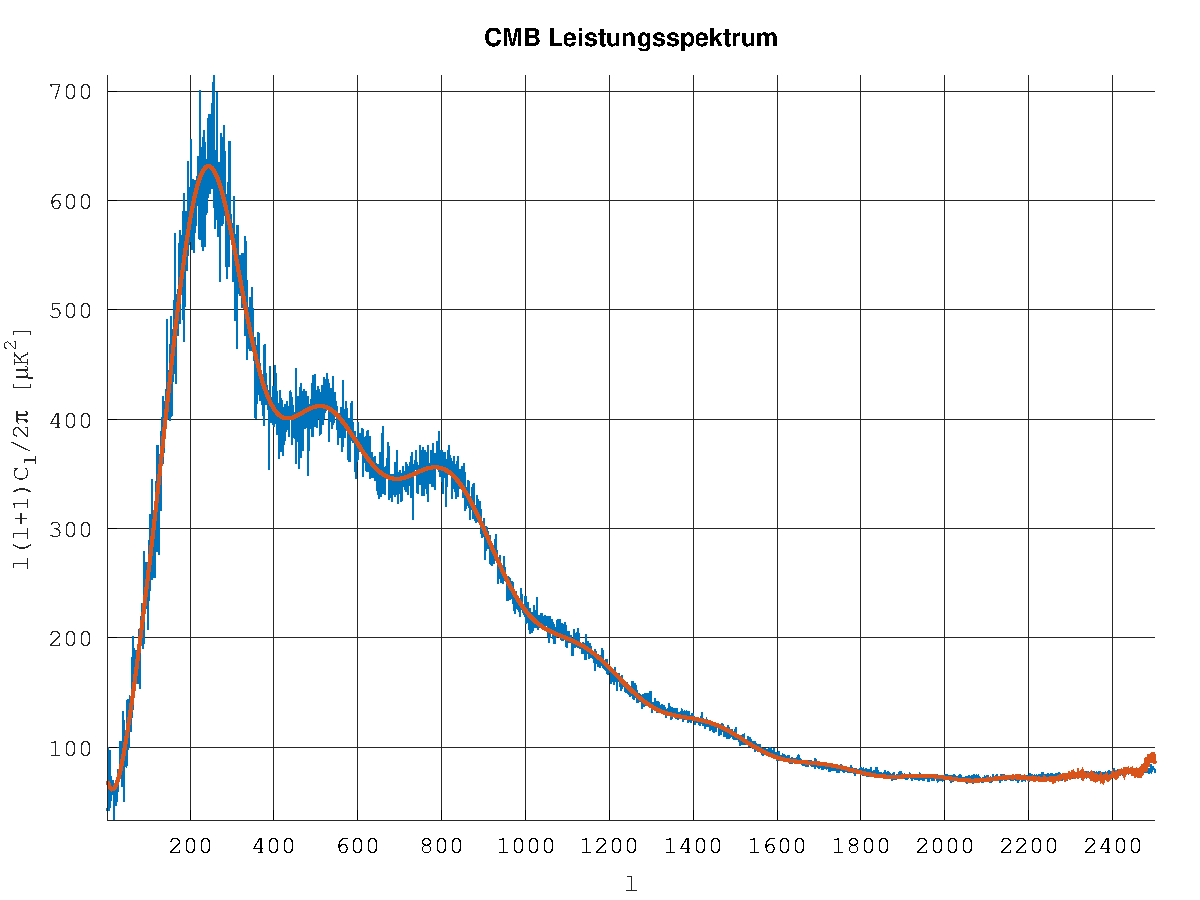
\includegraphics[width=\linewidth]{cmb/images/12k_2500.pdf}
	\caption{Leistungsspektrum berechnet bis zu $l = 2500$.}
	\label{fig:cmb-power-spec-2500}
\end{figure}

% TODO: Resultate zeigen